\chapter{Modelos de Aprendizagem Profunda}
\label{chap:redes-neuronais-convolucionais}

\section{Introdução}
\label{chap2:sec:intro}
O nosso cérebro processa constantemente o ambiente que nos rodeia. Durante todo o processo de aprendizagem e crescimento por que o ser humano passa, o cérebro cria regras que lhe permitem, entre muitas outras coisas, classificar objetos de forma quase instantânea. Este processo começa de forma supervisionada (os nossos pais classificam objetos, inicialmente desconhecido, por nós) levando a que criemos parâmetros que permitirão a identificação autónoma de futuras instâncias de qualquer objeto.\newline
\noindent 
\newline
\noindent Sabe-se que um neurónio recebe informação através das dendrites, processa o que recebeu e dispara um \textit{output} adequado. Trata-se, claramente, de uma simplificação daquele que é talvez um dos mecanismos mais fascinantes que a Ciência estuda. Contudo, serviu de base para que em 1943 o neurocientista  Warren McCulloch e o matemático Walter Pitts propusessem um neurónio artificial. A ideia base seria a mesma de um neurónio biológico, aliada à esperança de que muitas células simples seriam capazes de dar respostas complexas. 

\begin{figure}[h]
\centering
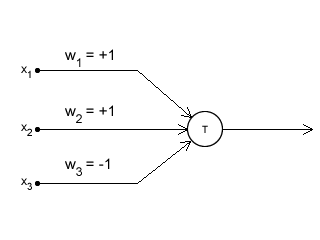
\includegraphics[width=155pt]{mp_neuron.png}
\caption{Modelo do neurónio artificial proposto por McCulloch e Pitts \cite{neuron_site}.}
\label{fig:mp_neuron}
\end{figure}

\section{Córtex Visual Primário}
\label{chap2:sec:cortex_visual}
Situado no Lobo Occipital, o Córtex Visual Primário (V1) é, a nível da visão, uma das regiões mais estudadas do cérebro. Sendo extremamente especializado na análise de objetos tanto em movimento como estáticos, possui um alto grau de reconhecimento de padrões.

\begin{figure}[h]
\centering
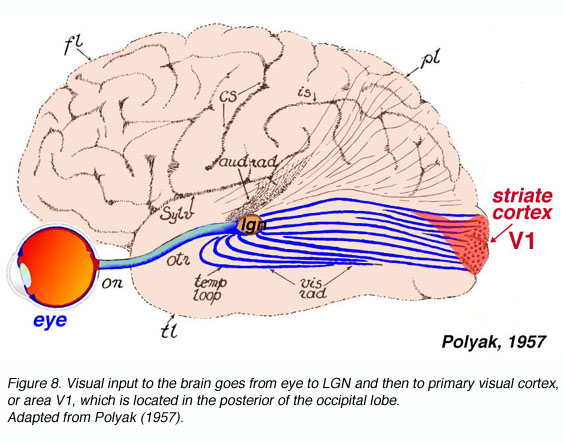
\includegraphics[width=150pt]{cortex.jpg}
\caption{Fluxo de informação desde o olho até ao Córtex Visual Primário \cite{cortex_site}.}
\label{fig:cortex}
\end{figure}

\noindent No decorrer do processamento de informação (figura \ref{fig:cortex}), o \textit{input} visual é obtido pela retina, com intervenção das suas células ganglionares, cones, bastonetes, células horizontais, células bipolares e células amácrinas. As terminações das células ganglionares agregam-se e surgem na parte posterior do olho já sob a forma do nervo ótico. A continuação deste nervo crucial para a Via Visual Primária, denominada de trato ótico, transporta a informação sensorial até ao \ac{NGL} - localizado no Tálamo, um importante centro nervoso.

\noindent Algum processamento é realizado nesta secção, destacando-se as células M (\textit{Magnocellular}), P (\textit{Parvocellular}) e K (\textit{Koniocellular}). Existem funções bem definidas e um grau de especialização diferenciador: os neurónios M são particularmente afetos à deteção de movimento; os neurónios P às caraterísticas espaciais (tamanho e forma) e os neurónios K a alguns aspetos da visão cromática.

\begin{figure}[h]
\centering
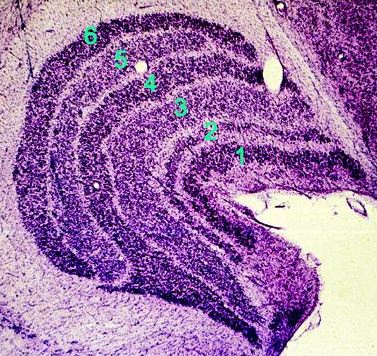
\includegraphics[width=115pt]{m_p_k_cells.jpg}
\caption{As seis camadas que compõe o \ac{NGL}: 1-2 (células M); 3-6 (células P) e as células K situam-se em zonas intermédias \cite{cells}.}
\label{fig:via_visual}
\end{figure}

\noindent Finalmente, esta informação filtrada e levemente tratada chega ao seu destino, o Córtex Visual Primário.

\noindent A partir dos estudos de Hubel e Weisel na década de 1960, foi possível perceber que os neurónios em V1 são excitados por caraterísticas tanto simples como complexas da imagem a ser analisada. Algumas células respondem melhor a arestas com um determinado ângulo (preferência de orientação), enquanto outras processam a informação vinda dos dois olhos de forma diferente (preferência ocular). Deste modo, a estrutura interna do Córtex Visual Primário é composta por colunas de neurónios com funções e reações a \textit{inputs} semelhantes.

\noindent Acredita-se que outras áreas envolventes a V1 desempenham um papel importante no processamento dos estímulos visuais. Porém, existem ainda muitos mistérios por desvendar e que continuarão a motivar a comunidade científica.

\begin{figure}[h]
\centering
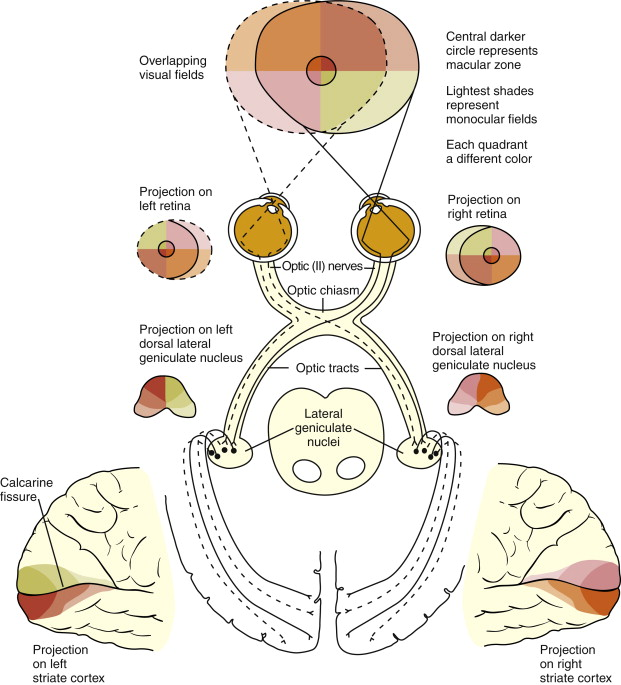
\includegraphics[width=325pt]{via_visual.jpg}
\caption{Vários componentes envolvidos no processamento de informação visual \cite{via_visual_primaria}.}
\label{fig:via_visual}
\end{figure}

\section{Redes Neuronais Convolucionais}
\label{chap2:sec:funcionamento}
Apresentada a estrutura biológica que inspirou o investimento nas Redes Neuronais artificiais, importa descrever os mecanismos que levam uma CNN a conseguir replicar (com as devidas diferenças) o processo anteriormente descrito. \newline

\noindent Tipicamente, uma CNN tem as seguintes camadas: camada(s) convolucional(ais), camada(s) de \textit{pooling} e camada(s) de classificação (camada(s) completamente ligada(s)).

\subsection{Camada Convolucional}
\label{chap2:subsec:convolucional}
Esta camada procura detetar \textit{features} de baixo nível, como arestas e curvas. Para tal, é usado um filtro (também chamado de \textit{kernel}). Uma imagem tem sempre a forma NxMxC, sendo N o número de linhas, M o número de colunas e C o número de canais de cor. De modo a diminuir o tamanho potencialmente inviável do \textit{input}, o \textit{kernel} (nada mais que uma matriz) passa pela imagem um número permitido de vezes - numa matriz 5x5 e com passo/\textit{stride} igual a 1, o \textit{kernel} cobre-a nove vezes originando um mapa de ativação 3x3 (figura \ref{fig:kernel}).


\noindent Note-se que outras etapas podem ser acrescentadas ao output da camada convolucional (por exemplo, a função de ativação ReLU promove não-linearidade, algo desejável quando se trabalha com imagens que não são lineares, por natureza) 

\begin{figure}[h]
\centering
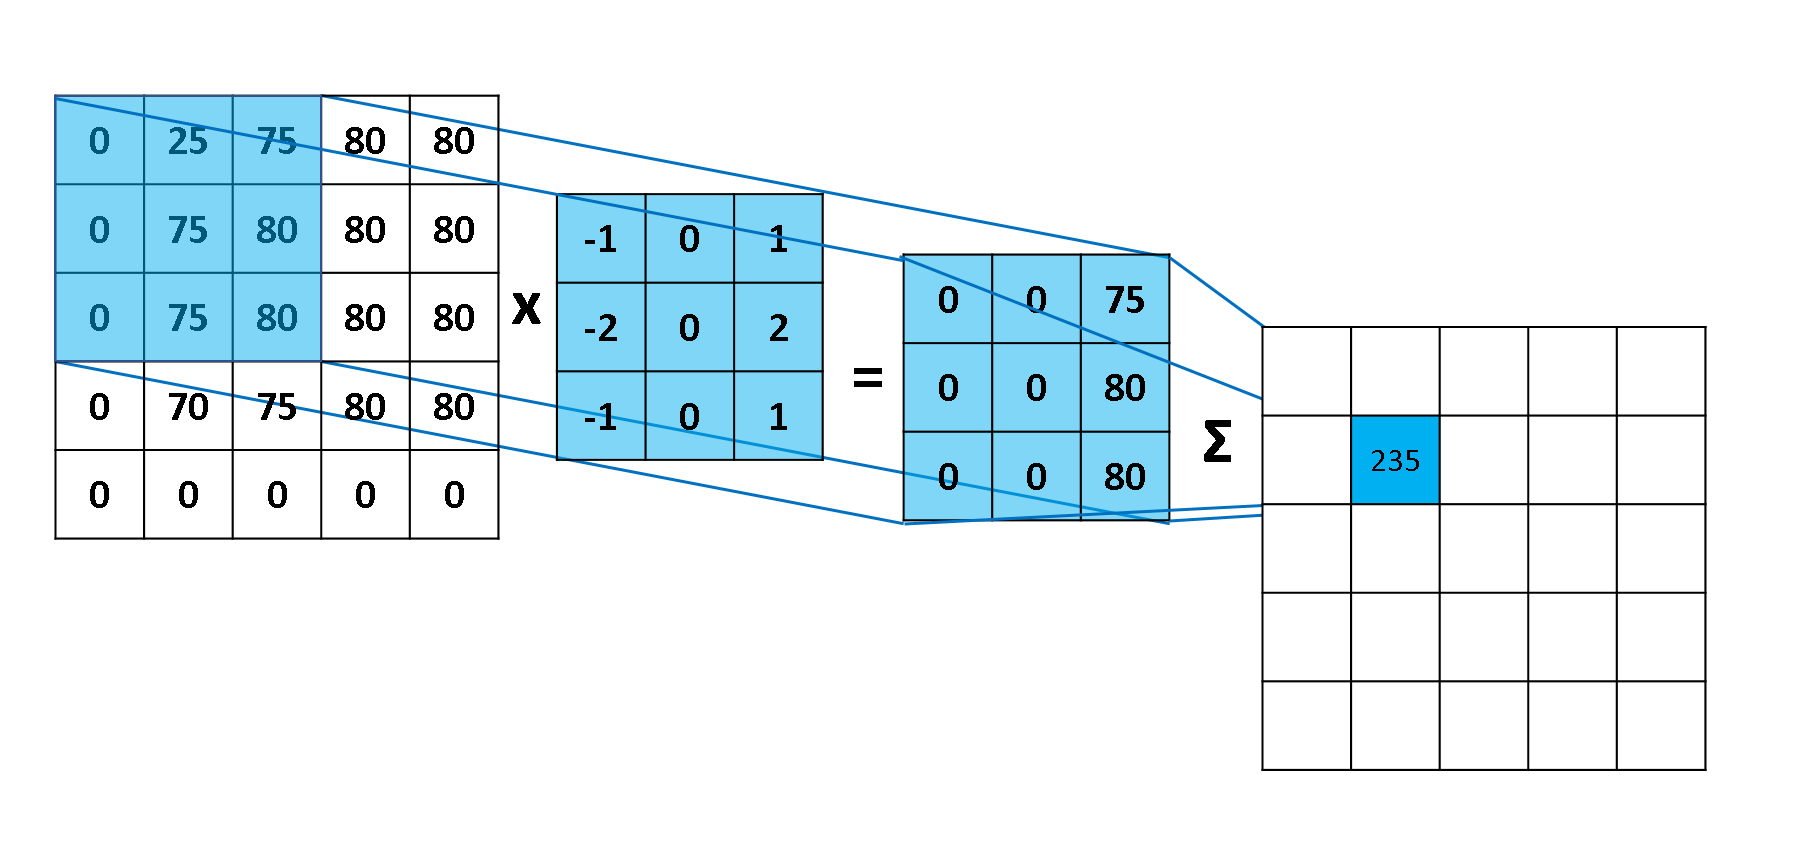
\includegraphics[width=350pt]{kernel.png}
\caption{Operação de convolução entre uma matriz de entrada 5x5 e um \textit{kernel} 3x3 \cite{kernel}.}
\label{fig:kernel}
\end{figure}

\noindent Os valores do \textit{kernel} são multiplicados com os da área abrangida na matriz inicial, sendo posteriormente somados (a matriz com todos estes números calculados contém as chamadas \textit{convolved features}).

\noindent O exemplo retratado na figura \ref{fig:kernel} representa uma simplificação do processo de convolução. Na realidade, podem-se considerar situações adicionais:

\begin{enumerate}
        \item No caso de uma imagem a cor RGB, existem três canais, pelo que a matriz de \textit{input} tem profundidade igual a 3. O \textit{kernel} é aplicada a cada canal e os três valores resultantes de cada canal são somados, dando, finalmente, o valor que entrará na matriz das \textit{convolved features}.
    \item De modo a extrair mais \textit{features}, podem ser utilizados vários \textit{kernels} com pesos diferentes. Assim, obtém-se um volume no fim desta camada, e não um \textit{output} com profundidade igual a 1.
\end{enumerate}

\subsection{Camada de \textit{Pooling}}
\label{chap2:subsec:pooling}
\noindent Sendo aplicada ao \textit{output} da etapa anterior, a camada de \textit{pooling} tem a função de reduzir a dimensão espacial das \textit{convolved features}, sem perder informação necessária à classificação. Esta camada é, ainda, capaz, de extrair \textit{features} dominantes em certas regiões da imagem de entrada. Consideram-se dois tipos de \textit{pooling}: \textit{max pooling} e \textit{average pooling}.\newline
\noindent A técnica de \textit{max pooling} opta por, a partir de uma região definida na matriz das \textit{convolved features}, escolher o maior valor possível (figura \ref{fig:pooling}). Apresenta a vantagem de reduzir possível ruído e combater o problema de \textit{overfitting} - manifesta-se quando os resultados no conjunto de teste são muito bons, mas a mesma \textit{performance} não se verifica nos exemplos de teste. \newline
\noindent Numa abordagem alternativa, \textit{average pooling} faz a média aritmética simples dos valores abrangidos pelo filtro escolhido, normalmente 2x2 e com passo/\textit{stride} semelhante (figura \ref{fig:pooling}). \newline
\noindent Comparando as duas variantes, \textit{max pooling} é a mais popular, sendo creditada como a melhor em termos de \textit{performance}.

\begin{figure}[h]
\centering
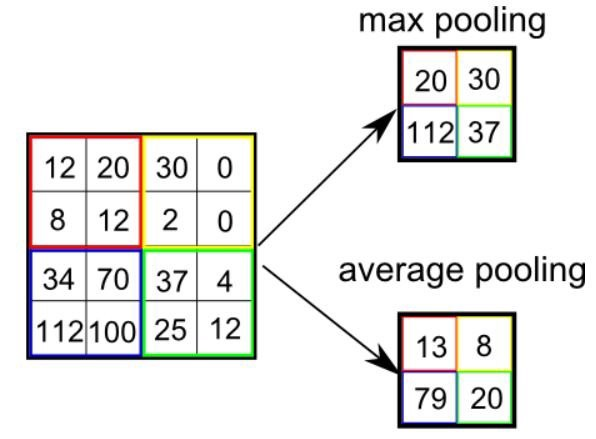
\includegraphics[width=185pt]{pooling.jpg}
\caption{2 tipos de \textit{pooling} \cite{pool}.}
\label{fig:pooling}
\end{figure}

\noindent Dependendo da aplicação e \textit{dataset} a analisar, podem ser usadas várias camadas convolucionais e de \textit{pooling} intercaladas.

\subsection{Camada Completamente Ligada}
\label{chap2:subsec:fully}
Em qualquer caso, o volume (matriz com profundidade) resultante da intercalação das camadas anteriormente mencionadas, será achatado na forma de um vetor coluna. Deste modo, é possível fornecer tal vetor, como \textit{input}, a uma rede neuronal tradicional (sendo que os neurónios de cada camada estão ligados com todos os da camada seguinte). Pode-se dizer que as camadas anteriores extraíram \textit{features} da imagem de entrada, enquanto que as camadas que se seguem classificam tudo o que foi obtido (dando mais importância a determinados padrões e formas que outros).

\noindent Na figura \ref{fig:fully}, os círculos amarelos representam o resultado da interpolação de "n" camadas de convolução e \textit{pooling}. Os círculos azuis agem como uma rede neuronal (tipicamente um \ac{MLP}) com tantas camadas escondidas quantas as necessárias para o problema a ser tratado. Finalmente, a última camada (vermelha), contém os neurónios ligados às classes existentes. É comum usar-se a função \textit{softmax} para obter uma distribuição probabilística sobre os \textit{outputs} finais da CNN.\newline

\begin{figure}[h]
\centering
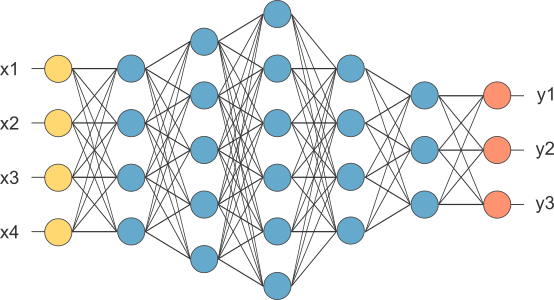
\includegraphics[width=330pt]{fully.png}
\caption{Visualização das camadas finais de uma CNN \cite{fully}.}
\label{fig:fully}
\end{figure}

\subsection{Função de \textit{Loss}}
\label{chap2:subsec:loss}
Uma função de \textit{loss} mede a performance de um modelo de classificação. No caso mais concreto dos problemas trabalhados, foi usada a função \textit{Cross-Entropy}. Apresenta a seguinte fórmula:

\begin{equation}
 H_{p}(q) = -\frac{1}{N}\sum_{i=1}^{N}y_{i}\log(p(y_{i}))+(1-y_{i})\log(1-p(y_{i}))
 \label{eq:eq_log}
\end{equation}

\noindent Na fórmula \ref{eq:eq_log}, \emph{$y_{i}$} representa a classe verdadeira de um dado ponto \emph{i}, N o número de pontos/elementos a classificar e \emph{$p(y_{i})$} a probabilidade de o ponto ser da classe 1. Numa análise à fórmula, se o ponto for da classe 1 (aplica-se em problemas binários, logo as classes são 1 e 0), o segundo termo anula-se e fica apenas \emph{$log(p(y_{i}))$}. Relembrando a curva logarítmica, uma probabilidade alta faria o termo ser próximo de 0 (aproximando-se pelos valores negativos). \newline 
\noindent De forma inversa, um ponto de classe 0 anula o primeiro termo e resulta em \emph{$log(1-p(y_{i}))$}. Como é de classe 0, a probabilidade de ser de classe 1 é, idealmente, baixa. Logo o valor dentro do logaritmo será próximo de 1 e a imagem respetiva, na função logarítmica, próxima de 0.\newline
\noindent Por fim, é invertido o valor resultante do somatório (os logaritmos de cada ponto resultaram em valores negativos) e feita a média das entropias cruzadas obtidas (\emph{$\frac{1}{N}$}).

\subsection{Notas finais}
\label{chap2:subsec:notas}
Nos últimos 20 anos, várias arquiteturas para \ac{CNN}s foram propostas, destacando-se as seguintes:

\begin{enumerate}
    \item \textbf{LeNet-5}, proposta por Yann LeCun em 1998, propunha-se a classificar dígitos, escritos à mão, digitalizados com uma resolução de 32x32 em escala de cinza.
    \item \textbf{AlexNet}, descrita por Alex Krizhevsky num \textit{paper} publicado em 2012, venceu a \ac{ILSVRC} do mesmo ano com uma vantagem de mais de 10\% para o segundo lugar. Conta com cinco camadas convolucionais (algumas seguidas de camadas de \textit{pooling}) e três camadas completamente ligadas. Propõe, ainda, o uso da função de ativação ReLU. Esta arquitetura demonstrou como a profundidade de uma rede é crucial para o desempenho final, bem como, técnicas de aumento de dados (espelhar ou cortar imagens) e de \textit{dropout} (remover neurónios aleatoriamente) ajudam a combater o problema de \textit{overfitting}.
    \item \textbf{GoogleNet/Inception}, vencedora da \ac{ILSVRC} de 2014 com um erro top-5 de 6.67\% (entrando no nível de performance do próprio ser humano). Conta com 22 camadas, vários módulos Inception (fazem várias convoluções e \textit{pooling}) e reduz o número de parâmetros da AlexNet (60 milhões) para apenas 4 milhões.
    \item \textbf{VGGNet}, perdeu em 2014 para a GoogleNet, sendo creditada pela capacidade de extração de \textit{features}. Como desvantagem, contém 138 milhões de parâmetros.
    \item \textbf{ResNet}, vencedora da  \ac{ILSVRC} de 2015, possui 152 camadas. Note-se que, mesmo assim, possui menor complexidade que a VGG.
\end{enumerate}

\noindent Devido à reconhecida capacidade de classificação de imagens, foi usada uma \ac{CNN} (mais concretamente, a arquitetura Inception) com vista a solucionar os dois problemas descritos nos capítulos seguintes.